\documentclass{article}

\usepackage{lipsum}
\usepackage{comment}
\usepackage[margin = 1in, includefoot]{geometry}

%Biblography Preamble
\usepackage[numbers,sort&compress]{natbib}

%\usepackage[hidelinks]{ hyperef } %this will help in hiding the links as if it is not done then links will appear in funky colors which won't look nice.

%Graphics Preamble
%\usepackage(graphicx) %Allows you to import images
%\usepackage(float) %Allows for control of float positions

%Bullet Preamble
\renewcommand{\labelitemi}{$\bullet$}
\renewcommand{\labelitemii}{$\diamond$}
\renewcommand{\labelitemiii}{$\circ$}



%Header and Footer stuff
\usepackage{fancyhdr}
\pagestyle{fancy}
\fancyhead{}
\fancyfoot{}
\fancyfoot[R]{\thepage\ }
\renewcommand{\headrulewidth}{0pt}
\renewcommand{\footrulewidth}{1pt}

%Header and Footer stuff over



\begin{document}

%commenting using package
\begin{comment}
this is used to comment out lines.
\title{Robust Anti-Spoofing Algorithm}
\author{Innovative Coder}
\date{August 27, 2017}
\maketitle
above written code will print t he report in very lame format 
the code written below is improved.
\end{comment}
%commenting over
\begin{titlepage}

	\begin{center}
	\line(1,0){300}\\
	[0.25 in]
	\huge{\bfseries Anti-Spoofing Algorithm}\\
	[2mm]
	\line(1,0){200}\\
	[1.5mm]
	\textsc{\LARGE Northern India engineering college}\\
	[0.75mm]
	\textsc{\Large -Affiliated to GGSIPU}\\
	[12.5cm]
	\end{center}
	
	\begin{flushright}  %flushright is used as the reference in the right hand border of the title page giving all sort of information about the researcher of the particular paper.
	\textsc{\large Jasneet Singh Sawhney\\
	\#IEEE member ID - 94379222\\
	August 27, 2017\\}
	\end{flushright}

\end{titlepage}

%Front matter 
\pagenumbering{roman}
\section*{Summary} %*the asterisk sign is used to remove the  heading number from it.
\addcontentsline{toc}{section}{\numberline{}Summary} %adding Summary to the table of contents
This is the summary of the complete research paper in order to help the reader go through the paper easily.
\cleardoublepage

\section*{Acknowledgements}
\addcontentsline{toc}{section}{\numberline{}Acknowldgements}
Thanks to IEEE department to give me chance to work on this project.
\cleardoublepage
%Table of contents
\tableofcontents   %this will require to be built twice as it take a couple of references to get built

%the contents page usually don't have the page number written on it, so we should get rid of the page number for this page
\thispagestyle{empty}
\cleardoublepage %to push the rest of matter on the next page
% This is the main body
\listoffigures
\addcontentsline{toc}{section}{\numberline List of Figures} 
\cleardoublepage

%\listoftables
%\addcontainsline{toc}{section}{\numberline{} List of tables}
%\cleardoublepages 

\pagenumbering{arabic}
\setcounter{page}{1}


\section{Introduction}\label{sec:intro}
This is the Robust Anti Spoofing Algorithm implementation using various algorithms.

The code is well explained.
\lipsum[1]

\newpage %new page is selected and matter is written to the new page
\section{LBP : Local Binary Pattern}
LBP is an intelligent way of checking the illumination. \cite{ref:Spoof_two,ref:three,ref:Spoof}

The introduction of this algorithm is found on page \pageref{sec:intro}

%Here we insert our figure
%\begin{figure}[H]
%	\centering
%	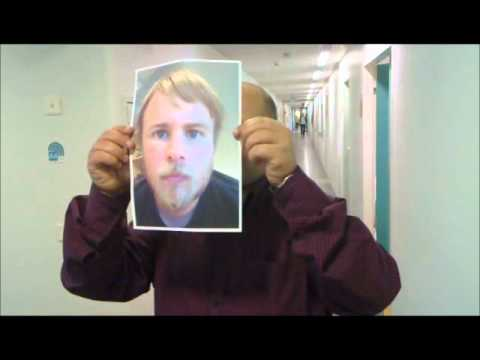
\includegraphics[height = 3in]{/Users/DBRSJ/Desktop/LaTeX/LaTeX_tutorial/Spoofing.png}
%	\caption[Optional caption]{Real, local caption} %if you want to insert a reference always give that in real curly braces otherwise it may cause problem in biblography
%	\label{fig:Spoofing}
%\end{figure}

%Figure \ref{fig:Spoofing}shows the spoofing of fingerprint


%Figure \ref{fig:spoofing}


\subsection{How it works?}
The pattern is described by an illumination matrix which is  taken as relative to the central grid.
%Our first table
%\begin{table}[H]
%	\centering
%	\label{tab:LBPworking}
%	\caption[This is optional caption,without reference]{Local caption, with reference}
%	\begin{tabular}{ | c r }
%		\bfseries{Grid number} & pattern generated?  & LBP?\\ \hline
%		3,2 & Yes & 1001101\\
%		6,8 & Yes & 1001010\\
%		9,8 & Yes & 1011100\\
%	\end{tabular}
%\end{table}
	
%Table \ref{tab:LBPworking} best approach for liveness detection.

\subsubsection{Subsubsection}\cite{ref:Spoof_two}
This is a sub subsection.

This sub subsection will be used for containing a list!

\begin{itemize}
	\item This is our first line
	\item This is second line and I am making it longer so that you can see how text wraps automatically in LaTeX.
	\begin{itemize}
		\item A bullet within a bullet.
			\begin{itemize}
				\item Must go deeper
			\end{itemize}
		\item[Title] A second one too. %the thing in [ ] will replace the bullet
 	\end{itemize}
	\item Good things comes in three.
	\item [Title] alpha beta gamma!!
	\item[This is a longer title] Beta gamma depta theta. 
		\begin{enumerate} % for a numbered list
			\item Some people
			\item Like lists with numbers instead.
		\end{enumerate}
\end{itemize}


\cleardoublepage
\bibliographystyle{IEEEtran} %biblography built using Bibdesk came along with the LaTeX package
\bibliography{/Users/DBRSJ/Desktop/LaTeX/LaTeX_tutorial/References/Spoof_ref.bib}
\addcontentsline{toc}{section}{\numberline{}References}
\cleardoublepage\

%Appendix starts here
\appendix
\section{LBP approach}
This is the appendix.


\end{document}